Neural networks are a class of supervised machine learning algorithms used for various learning and inferential tasks.  The first practical neural net was the perceptron proposed by Rosenblatt in 1958 \cite{Rosenblatt58theperceptron} who was inspired by earlier work of McCulloch and Pitts \cite{McCulloch-Pitts}.  More recently we have seen many exciting advances in the use of neural networks, including deep learning, reinforcement learning, and the use of Neural nets for transfer learning.
Here we will briefly discuss a basic neural network architecture, the multilayer perceptron, and the typical method for training neural nets, back propagation.  Because of the techniques use to make inference, neural networks that use the processes described here are called \textit{feedforward} neural networks.
%basic neural nets
\subsection{Single Layer Perceptron}
As first conceived by Rosenblatt, the perceptron was intended to be a machine, rather than a program. To this end, the inputs are intended to be binary vectors, and the output is also binary.  Shortly after Rosenblatt described the algorithm for the perceptron, Minsky and Papert \cite{Minsky90Perceptron} showed that a single perceptron is unable to calculate the XOR function.  While this proved that a single perceptron is not good for general computation, it turns out that a more general form, the multi layer perceptron, is a provably universal function approximator, as shown by Hornik \cite{HORNIK1991251} and expanded on by Lesho \textit{et. al.} \cite{LESHNO1993861}.  We start with the regular perceptron as a simplified example.

The perceptron is a type of linear discriminant.  Inspired by one model of human neurons, it is `on' if the output is large enough, and `off' otherwise.  The output is determined as a linear combination of data features.  A figure of a simple perceptron is seen in figure \ref{fig:perceptron}

\begin{figure}[ht]
  	\centering
  	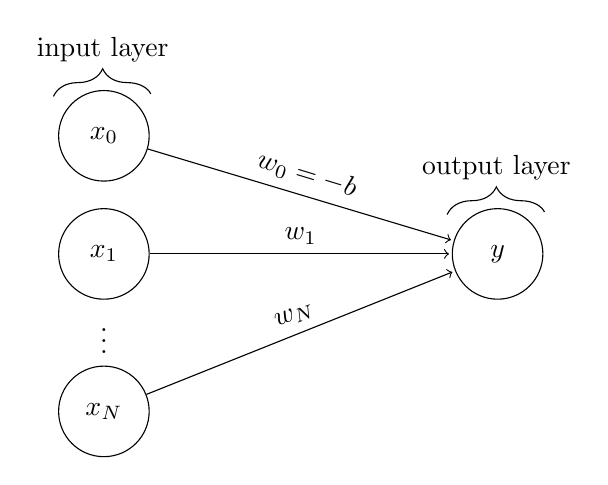
\begin{tikzpicture}[shorten >=1pt]
  	\tikzstyle{unit}=[draw,shape=circle,minimum size=1.15cm]
  	
  	\node[unit](x0) at (0,3.5){$x_0$};
  	\node[unit](x1) at (0,2){$x_1$};
  	\node(dots) at (0,1){\vdots};
  	\node[unit](xn) at (0,0){$x_N$};
  	
  	\node[unit](y1) at (5,2){$y$};
%  	\node(dots) at (4,1.5){\vdots};
%  	\node[unit](yk) at (4,0.5){$y_K$};
  	
  	\draw[->] (x0) -- node[above, rotate = -17]{\( w_0 = -b \)} (y1);
%  	\draw[->] (x0) -- (yk);
  	
  	\draw[->] (x1) -- node[above]{\( w_1 \)}(y1);
%  	\draw[->] (x1) -- (yk);
  	
  	\draw[->] (xn) -- node[above, rotate = 20]{\( w_N \)}(y1);
%  	\draw[->] (xn) -- (yk);
  	
  	\draw [decorate,decoration={brace,amplitude=10pt},xshift=-4pt,yshift=0pt] (-0.5,4) -- (0.75,4) node [black,midway,yshift=+0.6cm]{input layer};
  	\draw [decorate,decoration={brace,amplitude=10pt},xshift=-4pt,yshift=0pt] (4.5,2.5) -- (5.75,2.5) node [black,midway,yshift=+0.6cm]{output layer};
  	\end{tikzpicture}
  	\caption[Network graph of a perceptron with $N$ input units.]{The perceptron consists of $N$ input units and at least one output unit. All units are labeled according to their output: $y = H(z)$ in the case of the output unit; $x_n$ in the case of input units. The input values $x_n$ are propagated to the output unit using a weighted sum, in other words \( z = \bm w^{\intercal}\bm x \). An additional input value $x_0 := 1$ is used to include the biases as weights.}
  	\label{fig:perceptron}
\end{figure}

To describe this more precisely, let $\bm{X}=\{\bm x_n\}_{n=1}^{N}$ be the data, and \( \bm{T} =\{t_n\}_{n=1}^{N},\; t_n\in \{0,1\} \;\forall n \) be the labels. We will refer to the points \( \{(x^n,t^n)\}\subset\bm{X}\times \bm{T} \) as the training set. Then the perceptron algorithm seeks to determine the class of a new data point \( \bm x \) by using a function of the form
\begin{equation}\label{perceptron}
y = H(\bm w^{\intercal} \bm x).
\end{equation}
Here \( \bm w \) is a vector of real weights determined through training and  \( H(v) \) is the Heaviside step function
\[ H(v) =\begin{cases}
 			1 &\text{ if }v\geq 0\\
 			0 &\text{ if }v<0
		 \end{cases} 
\]

In practice, a bias term \( b \) is added to equation \ref{perceptron}, so that it becomes \( y = H(\bm w^{\intercal} \bm x +b) \). This is most usually done by adding an extra feature to all of our data points while training. This extra feature is always set to 1.  An additional weight is also appended to the weight vector \( \bm w \) so that the model still looks like \ref{perceptron}. The effect of bias is to change where the perceptron activates, and makes it harder to `fire' (\textit{i.e.} give a positive output for a given input). This also has the effect of allowing the model to center the data, as would happen with a bias in the regression setting.

%talk a bout finding weight vis gradient descent, this is easier w/ smooth activation lead into logit
The act of training for a perceptron is choosing weights \( \bm w \) so that \( H(\bm w^{\intercal} \bm x_n) = t_n\;\forall (x_n,t_n)\in \mathcal{X}\times \mathcal{T} \). The hope is that this will generalize well to new data points.  The point emphasized in the Minsky book \cite{Minsky90Perceptron} is that training will only work if the two classes in the training set are linearly separable.  This only applies to single layer perceptrons, as one can create a NAND gate from a single layer perceptron, so using multiple perceptrons one could conceivably approximate any function to arbitrary precision.

%single layr as logit regression
%\subsection{Single Layer Network as Logistic Regression}
The perceptron algorithm also includes methods for training, but these are not in common use today.  More modern architecture use the backpropagation algorithm, which requires gradient descent.  The problem with perceptrons in that context is that the derivative of the Heaviside step function is zero. 

The use of the Heaviside function in the perceptron is called an activation function.  In more modern neural networks, activation functions with non-zero derivative allow use of backpropagation and gradient descent.  The discussion in section \ref{logisticReg} mentions the sigmoidal activation function.  As discussed there, if we replace the Heaviside step function with the sigmoid function, then we are actually performing logistic regression.  We will refer to perceptrons using the sigmoidal activation function as sigmoidal neurons.

%multi-layer multiclass network
\subsection{Multilayer Perceptron as a Multi-Class Classifier}
The multilayer perceptron (MLP) is actually built out of several sigmoidal neurons.  The MLP we describe has a single hidden layer, which means that the output of one sigmoidal neuron becomes the input for the next neuron.  Figure \ref{fig:MLP} below gives an example of a single hidden layer MLP.

\begin{figure}[ht]
	\centering
	\begin{tikzpicture}[shorten >=1pt,->,draw=black!50, node distance=\layersep]
	\tikzstyle{every pin edge}=[<-,shorten <=1pt]
	\tikzstyle{neuron}=[circle,fill=black!25,minimum size=17pt,inner sep=0pt]
	\tikzstyle{input neuron}=[neuron, fill=green!20];
	\tikzstyle{output neuron}=[neuron, fill=red!20];
	\tikzstyle{hidden neuron}=[neuron, fill=blue!20];
	\tikzstyle{annot} = [text width=4em, text centered]
	
	% Draw the input layer nodes
	\foreach \name / \y in {1,...,5}
	% This is the same as writing \foreach \name / \y in {1/1,2/2,3/3,4/4}
	\node[input neuron] (I-\name) at (0,-\y) {\(x_\y\)};
	
	% Draw the hidden layer nodes
	\foreach \name / \y in {1,...,6}
	\path[yshift=0.5cm]
	node[hidden neuron] (H-\name) at (\layersep,-\y cm) {\(z_\y\)};
	
	% Draw the output layer nodes
	\foreach \name / \y in {1,...,3}
		\node[output neuron,pin={[pin edge={->}]right:\(\hat{y}_\y\)}] (O-\name) at (2*\layersep,-1 cm-\y cm) {\(y_\y\)};
	
	% Connect every node in the input layer with every node in the
	% hidden layer.
	\foreach \source in {1,...,5}
	\foreach \dest in {1,...,6}
	\path (I-\source) edge (H-\dest);
	
	% Connect every node in the hidden layer with the output layer
	\foreach \source in {1,...,6}
	\foreach \dest in {1,...,3}
	\path (H-\source) edge (O-\dest);
	
	% Annotate the layers
	\node[annot,above of=H-1, node distance=1cm] (hl) {Hidden layer};
	\node[annot,left of=hl] {Input layer};
	\node[annot,right of=hl] {Output layer};
		
	\end{tikzpicture}
		\caption[Network graph of a multilayer perceptron.]{A graph model of a single hidden layer MLP with 5 inputs, 3 output and 6 hidden layer nodes. The output of each layer is determined by composing a linear map with a nonlinear map. The general form of this nonlinear map is determined at the outset, though it may have trained parameters. The linear map is determined through a set of learned weights.}
	\label{fig:MLP}
\end{figure}

Neural networks such as the MLP are often called feedforward neural networks.  This is because at each stage of computation information is only passed forward toward the output nodes.  The general pattern of feedforward nets is that each node passes a weighted sum of previous nodes through an activation function.  We have already mentioned two activation functions, Heaviside and sigmoidal. Other common activation functions are hyperbolic tangent, rectified linear unit (RELU), and sigmoid linear unit \cite{elfwingSiLU}.

In the case of the MLP, each of the hidden layer nodes work as a sigmoidal neuron \textit{i.e.} \( z_l = \gs(\bm w_{1l}^{\intercal}\bm x) \). Likewise, each of the output layers can be expressed as a sigmoidal neuron, \( y_k = \gs(\bm w_{2k}^{\intercal}\bm z) \). This view is not consistent with a desire to express the output in terms of a probability. This is particularly important if we wish to use the MLP as a multi-class classifier, as we wish to interpret the outputs as \( P(k_n=k|\bm x_n) \).

While each individual output is a log odds in the sense of logistic regression, together we cannot interpret each individual \( y_k \)  as a probability.  In particular, we have no guarantee that \( \sum_k y_k=1 \).  To fix this, we may pass the outputs \( y_k \) through the softmax function \textit{i.e.} 
\begin{equation}\label{MLPsoftmax}
\hat{y}_k = \frac{e^{y_k}}{\sum_{j=1}^{K} e^{y_j}}
\end{equation}

Passing the output through a softmax function has the effect of guaranteeing that \( \sum_k y_k=1 \), but if we are to interpret \( \hat{y}_k \) as a probability, then it must be regarded as a Gibbs distribution.  From a mathematical standpoint this changes the interpretation of \( y_k \) to an approximation of an energy function.  To be consistent with this interpretation, we must be careful in our choice of cost function.  This becomes more apparent when we consider the role of backpropagation in training.

\subsection{Backpropagation}\label{subsect:backprop}
Backpropagation (BP) was modernly popularized as a method for training neural networks by Rumelhart et. al. \cite{rumelhart1986learning} in 1986. Similar training methods had been used earlier, \textit{e.g.} Linnainmaa \cite{Linnainmaa1976}, in the context of optimization. Backpropagation for use in neural network training was first used by Paul Werbos in his 1974 thesis \cite{werbos1994roots}. Brief histories of the development of BP can be found in Griewank \textit{et.al.} \cite{griewank2008deriv}, Schmidhuber \cite{Schmidhuber_2015}, and Goodfellow \textit{et.al.},\cite[see ch6.6]{Goodfellow-et-al-2016}. The practical development and popularization of BP led to a very active period of research in multilayer neural networks.

While BP is often described as `just gradient descent', it is the case that BP actually refers to a specific method for calculating the gradient of the loss function with respect to the weights.  Backpropagation relies heavily on the chain rule, and the architecture of perceptron inspired neural networks. We will use a simple neural network model to help describe BP.  We draw most of the inspiration for this example from the book by Goodfellow  et. al. \cite[ch6.5]{Goodfellow-et-al-2016}

The goal of BP is to adjust the weights by subtracting off the gradient of the cost function with respect to the weights.  The key realization of BP is that with the correct network setup, this may be done by passing information backwards through the graph.  

Recall that the typical role of a layer in a feedforward neural net is to pass forward predictions based on information from the previous layer.  The role of layer \( \ell \) during training with backpropagation is to pass forward the predictions as usual. Then during the backward pass layer \( \ell \) updates its own weights \( W_{\ell} \) using gradient descent and the chain rule. Finally the layer passes back the new gradient of the loss with respect to the output \( \bm z_{\ell-1} \)of the previous layer.  Figure \ref{fig:backprop} gives a high level model of this process.

\begin{figure}[ht]
	\centering

%\usetikzlibrary{arrows}
\begin{tikzpicture}

\draw [ultra thick] (-2.5,2.5) rectangle (1.5,-1.5);
\node (v1) at (-7.5,1.5) {};
\node (v2) at (-2.4,1.5) {};
\node (v4) at (-2.4,-0.5) {};
\node (v3) at (-7.5,-0.5) {};
\node (v5) at (1.4,1.5) {};
\node (v6) at (6.5,1.5) {};
\node (v8) at (6.5,-0.5) {};
\node (v7) at (1.4,-0.5) {};
\draw  [->](v1) edge node[above]{\(\bm z_{\ell-1}\)}(v2);
\draw  [<-](v3) edge node[above]{\(\dfrac{\partial L}{\partial \bm z_{\ell-1}}=\dfrac{\partial L}{\partial \bm z_{\ell}}\dfrac{\partial \bm z_{\ell}}{\partial \bm z_{\ell-1}}\)}(v4);
\draw  [->](v5) edge node[above]{\(\bm z_{\ell} = \bm \sigma_{\ell}(\bm z_{\ell-1})\)}(v6);
\draw  [<-](v7) edge node[above]{\(\dfrac{\partial L}{\partial \bm z_{\ell}}\)}(v8);
\node at (-0.5,1.5) {\(\sigma_{\ell} = \bm f_{\ell}(\langle \bm W_{\ell}, \cdot \rangle)\)};
\node at (-0.5,-0.5) {\(\nabla_{\bm W_{\ell}}\sigma_{\ell} = \dfrac{\partial L}{\partial \bm z_{\ell}}\dfrac{\partial \bm z_{\ell}}{\partial \bm W_{\ell}}\)};
\node at (-0.5,3) {Layer $\ell$};
\end{tikzpicture}
	\caption[Conceptualized model of a single network layer.]{A model of a single layer in a neural network. For the feedforward pass it calculates  \(\bm z_{\ell} = \bm \sigma_{\ell}(\bm z_{\ell-1}) = \bm f_{\ell}(\langle \bm W_{\ell},\bm z_{\ell-1}\rangle) \).  On the backward pass it calculates \( \dfrac{\partial L}{\partial \bm W_{\ell}} \) and \( \dfrac{\partial L}{\partial \bm z_{\ell-1}} \). The layer uses \( \dfrac{\partial L}{\partial \bm W_{\ell}} \) to update its own weights with gradient descent. The layer passes \( \dfrac{\partial L}{\partial \bm z_{\ell-1}} \) to the previous layer to use.}
	
\label{fig:backprop}
\end{figure}

While the diagram in figure \ref{fig:backprop} implies that the backpropagation algorithm only uses chain rule, in reality it may be a bit more complicated.  Since \( \gs_{\ell}:\R^{d_{\ell-1}}\rightarrow \R^{d_{\ell}}\) is a non linear multivariate function, taking derivatives can be complicated.  Further, the parameters \( \bm W_{\ell} \) might be part of a higher dimensional linear map (e.g matrix, tensor). For such situations we need to be more careful in calculating gradients.  While many references address this problem, \cite{matGradChain} offers a good treatment of the chain rule in such situations. Section \ref{subsect:derivNotation} covers this in more detail.

Finally it is worth noting that in many situations, backpropagation can be simply calculated in a coordinate manner.  This is because much of the structure of neural nets gives an implied coordinate system to each layer.  It is also a good reason that one must be careful in the choice of cost function. When an appropriate cost function is chosen, backpropagation becomes a quick operation. This helps explain why backpropagation is so popular in recent neural net training.